\documentclass{ximera}

\input{../preamble.tex}

\title{Adding and subtracting with negative numbers}
\author{Vic Ferdinand, Betsy McNeal, Jenny Sheldon}

\begin{document}

\begin{abstract}
We look at adding and subtracting integers.
\end{abstract}
\maketitle

Now that we have our models ready, let's apply them to solve problems about addition and subtraction. 
As we begin this section, you may want to consider re-reading the sections about \link[adding and subtracting]{https://ximera.osu.edu/m4t/elementaryTeachersOne/elementaryReading/AdditionSubtraction/AddingAndSubtracting}. 
We'll be using these ideas throughout!

\section{Checks and Bills}

Let's begin with one of our most basic addition examples.
\begin{example}
Johnny has $9$ apples, and Suzy gives him $2$ more apples.  How many apples does Johnny have now?  

\begin{prompt}
Write an expression using the addition sign which solves this problem.  $\answer[given]{9} + 2$
\end{prompt}
\end{example}

If we change this example to a story about checks and bills, we might use the following instead.
\begin{example}
Johnny opens his business for today with a net worth of \$$9$, and then he receives a check for \$$2$.  What is Johnny's net worth now?
\begin{explanation}
Johnny begins with a net worth of \$$9$.  From our checks and bills model, we know that receiving something means we should \wordChoice{\choice[correct]{add the value to} \choice{subtract the value from}} Johnny's total net worth.  Since the object he receives is a check, the value should be \wordChoice{\choice[correct]{positive} \choice{negative}}.  Therefore, the expression we would write which solves this problem is $\answer[given]{9} + 2$. 

\end{explanation}
\end{example}

Notice that the first number in our expression is Johnny's starting amount and the second number is the amount of the check. In future examples we might leave either number blank, so be sure to follow this pattern in terms of which number is entered first.

Let's begin to include some negative numbers in our stories.
\begin{question}
Johnny opens his business for today with a net worth of \$$-8$, and then he receives a 
check for \$$4$.  What is Johnny's net worth now?
\begin{prompt}
Johnny's net worth is now $-8 + \answer[given]{4}$.
\end{prompt}
\end{question}

When Johnny receives a check, we expect his account balance to go up, and indeed our answer is larger than the starting amount.


\begin{question}
Johnny opens his business for today with a net worth of \$$-14$, and then he sends a check for \$$6$.  
What is Johnny's net worth now?

\begin{prompt}
As an expression involving the subtraction sign, Johnny's net worth is now $-14 \answer[given]{-} \answer[given]{4}$.
\end{prompt}
\end{question}
Sending a check should make Johnny's balance decrease, and indeed he ends up with less money than he started with.


\begin{question}
Johnny opens his business for today with a net worth of \$$-22$, and then he sends a bill for \$$54$.  
What is Johnny's net worth now?

\begin{prompt}
As an  expression, Johnny's net worth is now $\answer[given]{-22} \answer[given]{-} \answer[given]{-54}$.
\end{prompt}
\end{question}
In this last question, notice that Johnny is now sending a bill.  Since we assume this bill will be paid 
by the person to whom it was sent, Johnny's total net worth should be greater than it was at the 
beginning of the day. 

Notice that after each example, we took a moment to think about whether our answer was sensible in terms of how Johnny's balance increased or decreased during the story. It's important to notice that we are using the {\em story context}, not the fact that we are adding or subtracting, to decide whether the answer should be larger or smaller. We aren't making numbers larger by adding or smaller by subtracting -- either could be true! We also didn't need the rules we've memorized for using negative numbers, but could use our reasoning about what's happening in the story problem instead. 

Speaking of rules, you may have learned some rules about subtraction in the past.  In particular, you might be familiar 
with what happens when we subtract a negative number.  How can we make sense of what we already know, 
but in terms of checks and bills?
\begin{example}
When we subtract a negative number, our checks and bills method says we are 
\wordChoice{\choice{receiving} \choice[correct]{sending}} a 
\wordChoice{\choice{check} \choice[correct]{bill}}.  So, when writing such a story, we don't care what 
Johnny's net worth is at the beginning of the day.  Let's call it \$$A$.  Let's also say our bill is 
worth \$$B$.  We want to compute $A - (-B)$.  After the person to whom Johnny sent this bill pays, 
the result to Johnny will be that he has \$$B$ more than \$$A$.  So, we combine Johnny's original net 
worth \$$A$ with the additional amount \$$B$ to see that
\[
A - (-B) = \answer[given]{A + B}.
\]
\end{example}


Checks and bills story problems can feel repetitive, and sometimes people want to change up the story a little bit. If you move away from what we've done in these examples or write stories using other contexts, be sure to check your work carefully. In particular, asking the right question in your story problem can be the trickiest part. Here are some examples of questions to avoid.

\begin{example}
Johnny receives a check for \$$18$ and a bill for \$$14$.  What is Johnny's net worth now?
\begin{explanation}
We don't actually have enough information to answer this question, because we don't know what Johnny's net worth was when the day began.  If he began with a net worth of \$$10$, his new net worth is $\answer[given]{10 + 18 + (-14)}$.  If he began the day with \$$0$, his new net worth is $\answer[given]{0 + 18 + (-14)}$.  The second answer is likely what the writer of this question was aiming for, but we can't know for sure!
\end{explanation}
\end{example}

\begin{example}
Johnny starts the day with a net worth of \$$7$, and then sends a bill for \$$5$.  How much 
did Johnny's net worth change?
\begin{explanation}
This story looks very similar to some of our other stories, but if we read the question 
carefully, we see an important difference.  We are asked how much Johnny's net worth 
{\em changes}, so we do not need the information about his beginning net worth.  Our bill was for 
\$$5$, and he sent this bill to someone else, so his net worth changes by $\answer[given]{5}$.  
This is not a story problem for $7 - (-5)$.
\end{explanation}
\end{example}


However, there are ways to be more creative. 


\begin{question}
Johnny opens his business for today with a net worth of \$$-2$ and then the mail arrives.  Afterwards, 
Johnny's net worth is now \$$-7$.  What was the value of what Johnny received in the mail?

\begin{explanation}
In this example, we know that Johnny's starting balance is $-2$, so this would be the \wordChoice{\choice[correct]{first} \choice{last}} number in our expression. But the $-7$ is not what came in the mail, it's his ending balance. In other words, we might use the equation
\[
\answer[given]{-2} + ? = \answer[given]{-7}
\]
to model this situation. But when we solve for the question mark, we would use the expression
\[
-7 - (-2)
\]
instead. So this story problem correctly models $-7-(-2)$. In a sense, we are comparing Johnny's ending balance to his starting balance to find out what came in the mail.
\end{explanation}
\end{question}

Any time you write a story problem, it's an excellent practice to go back and try to answer the question from an objective perspective.  Is the question really asking what you intend?  Is there any other way the question could be interpreted?  Especially in class or on a homework assignment, ask someone else for their opinion!


\section{Number Lines}

Next, let's use a number line to solve some addition problems with integers.  You can write a story problem to go along with each of these addition problems for extra practice.

\begin{example}
Imagine using a number line like the one below to solve the addition problem $5 + 3$.
\begin{center}
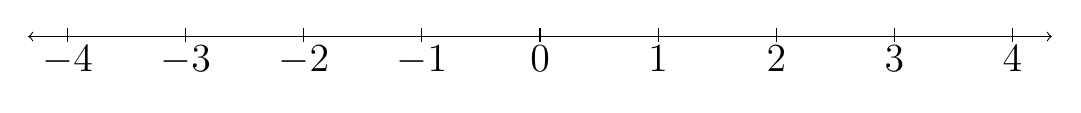
\begin{tikzpicture}[font=\Large]
\draw[<->] (-0.5,0) -- (12.5,0);
\foreach \x in {0,1.5, 3, 4.5, 6, 7.5, 9, 10.5,12}
\draw[shift={(\x,0)},color=black] (0pt,3pt) -- (0pt,-2pt);
\draw (0,0) node[below]{$-4$};
\draw (1.5,0) node[below]{$-3$};
\draw (3,0) node[below]{$-2$};
\draw (4.5,0) node[below]{$-1$};
\draw (6,0) node[below]{$0$};
\draw (7.5,0) node[below]{$1$};
\draw (9,0) node[below]{$2$};
\draw (10.5,0) node[below]{$3$};
\draw (12,0) node[below]{$4$};
\end{tikzpicture}  
\end{center}
We begin by standing on the number line at the tick marked with $\answer[given]{5}$.  Since we are adding, we move 
\wordChoice{\choice[correct]{forward} \choice{backward}}.  We will face 
\wordChoice{\choice[correct]{right} \choice{left}} since $3$ is positive and move $\answer[given]{3}$ spaces.  
Where on the number line are we now? 

\begin{prompt}
We are located at the tick labeled $\answer[given]{8}$.
\end{prompt}
\end{example}

When we started at $5$ and added $3$, we ended up further to the right on the number line, so our answer was larger than when we started.


\begin{example}
Imagine using a number line like the one below to solve the subtraction problem $-8 - 4$.
\begin{center}
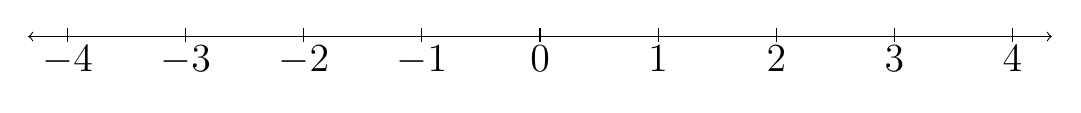
\begin{tikzpicture}[font=\Large]
\draw[<->] (-0.5,0) -- (12.5,0);
\foreach \x in {0,1.5, 3, 4.5, 6, 7.5, 9, 10.5,12}
\draw[shift={(\x,0)},color=black] (0pt,3pt) -- (0pt,-2pt);
\draw (0,0) node[below]{$-4$};
\draw (1.5,0) node[below]{$-3$};
\draw (3,0) node[below]{$-2$};
\draw (4.5,0) node[below]{$-1$};
\draw (6,0) node[below]{$0$};
\draw (7.5,0) node[below]{$1$};
\draw (9,0) node[below]{$2$};
\draw (10.5,0) node[below]{$3$};
\draw (12,0) node[below]{$4$};
\end{tikzpicture}  
\end{center}
We begin by standing on the number line at the tick marked with $\answer[given]{-8}$.  Since 
we are subtracting, we will move \wordChoice{\choice{forward} \choice[correct]{backward}}.  We 
will face \wordChoice{\choice[correct]{right} \choice{left}} since $4$ is positive, and move 
$\answer[given]{4}$ spaces.  Where on the number line are we now? 

\begin{prompt}
We are located at the tick labeled $\answer[given]{-12}$.
\end{prompt}
\end{example}

When we start at $-8$ and subtract $4$, we end up farther to the left on our number line, so our answer is smaller than when we started. This isn't only because we are subtracting, but because of the total package of our movement on the number line. Compare and contrast this example with the next one!


\begin{example}
Imagine using a number line like the one below to solve the subtraction problem $(-22) - (-54)$.
\begin{center}
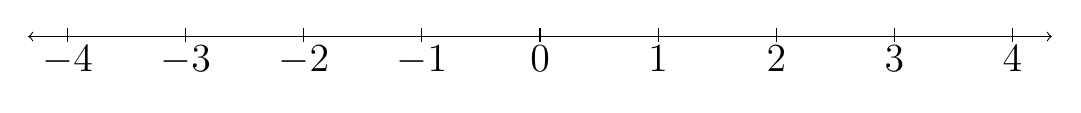
\begin{tikzpicture}[font=\Large]
\draw[<->] (-0.5,0) -- (12.5,0);
\foreach \x in {0,1.5, 3, 4.5, 6, 7.5, 9, 10.5,12}
\draw[shift={(\x,0)},color=black] (0pt,3pt) -- (0pt,-2pt);
\draw (0,0) node[below]{$-4$};
\draw (1.5,0) node[below]{$-3$};
\draw (3,0) node[below]{$-2$};
\draw (4.5,0) node[below]{$-1$};
\draw (6,0) node[below]{$0$};
\draw (7.5,0) node[below]{$1$};
\draw (9,0) node[below]{$2$};
\draw (10.5,0) node[below]{$3$};
\draw (12,0) node[below]{$4$};
\end{tikzpicture}  
\end{center}
We begin by standing on the number line at the tick marked with $\answer[given]{-22}$.  Since we 
are subtracting, we will move \wordChoice{\choice{forward} \choice[correct]{backward}}.  We 
will face \wordChoice{\choice{right} \choice[correct]{left}} since $54$ is negative and then move 
$\answer[given]{54}$ spaces.  Where on the number line are we now? 

\begin{prompt}
We are located at the tick labeled $\answer[given]{32}$.
\end{prompt}
\end{example}

Now, when we subtracted $-22$, we ended up farther to the right than our starting point, meaning our answer is larger than when we started. Subtraction can sometimes make things larger!


We can also use the previous example to investigate why subtracting a negative number gives us the same result as adding that number.  Using 
number lines, we can see that if we are subtracting, we are facing {\em left} while moving
{\em backward}.  The net result is the same as if we were facing right while moving forward. 
Try this out with some friends if you are skeptical.


\section{Red and black chips}

To model with red and black chips, we will use our meanings of addition and subtraction. However, 
sometimes we will need to make adjustments to what our starting value looks like so that we can 
correctly apply these operations.

\begin{problem}
Use red and black chips to model $7 + (-4)$.

\begin{explanation}
The expression $7 + (-4)$ tells us that we are starting with a value of \wordChoice{\choice{4} \choice{-4} \choice[correct]{7} \choice{-7}}. We can draw our starting value with any number of chips, but let's start with the most basic representation of $7$ black chips.

\begin{image}

\begin{tikzpicture}
	\foreach \x in {0, 1, 2, 3, 4, 5, 6} \draw[fill=black] (\x, 0) circle (4pt);
\end{tikzpicture}
\end{image}


We then want to \wordChoice{\choice[correct]{combine} \choice{take away} \choice{make groups}} because the expression is asking us to add. The value that we want to add is $-4$, and the most basic way to represent this value is by using \wordChoice{\choice{4 black chips} \choice[correct]{4 red chips} \choice{5 black chips and 1 red chip} \choice{5 red chips and 1 black chip}}. 

To finish the problem, we combine all of our chips together.
\begin{image}

\begin{tikzpicture}
	\foreach \x in {0, 1, 2, 3, 4, 5, 6} \draw[fill=black] (\x, 0) circle (4pt);
	\foreach \x in {0, 1, 2, 3} \draw[fill=red] (\x, -1) circle (4pt);
\end{tikzpicture}
\end{image}

We can cancel zero pairs of one red and one black chip, leaving us with a total value of $\answer[given]{3}$.

\end{explanation}
\end{problem}
In this example, we can see why adding a negative number gives us the same result as subtracting. When we place the red chips down on the table, they cancel out black chips in a one-to-one correspondence. We could almost think about the red chips as taking away the corresponding black ones from the total value of all of our chips. However, be careful to note that we modeled $7 + (-4)$ in this example, not $7 - 4$. Pause and draw a picture of $7-4$ in your notes, and then compare and contrast these two expressions.

\begin{problem}
Use red and black chips to model $6 - (-2)$.

\begin{explanation}
The expression $6 - (-2)$ tells us that we are starting with a value of \wordChoice{\choice[correct]{6} \choice{-6} \choice{2} \choice{-2}}. We can draw our starting value with any number of chips, but let's start with the most basic representation of $6$ black chips.

\begin{image}

\begin{tikzpicture}
	\foreach \x in {0, 1, 2, 3, 4, 5} \draw[fill=black] (\x, 0) circle (4pt);
\end{tikzpicture}
\end{image}


We then want to \wordChoice{\choice{combine} \choice[correct]{take away} \choice{make groups}} because the expression is asking us to subtract. The value that we want to subtract is $-2$, but now we have a problem. We want to take away $2$ red chips, but we don't have any red chips to remove. Luckily, we can represent our starting value of $6$ in many ways. In order to have enough chips to take away these $2$ red, the most efficient way to represent a total value of $6$ is to use \wordChoice{\choice{6 black chips} \choice{6 red chips} \choice{7 black chips and 1 red chip} \choice[correct]{8 black chips and 2 red chips} \choice{9 black chips and 3 red chips}}. Let's pause and draw this situation.

\begin{image}

\begin{tikzpicture}
	\foreach \x in {0, 1, 2, 3, 4, 5, 6, 7} \draw[fill=black] (\x, 0) circle (4pt);
	\foreach \x in {8, 9} \draw[fill=red] (\x, 0) circle (4pt);
\end{tikzpicture}
\end{image}

To finish the problem, we take away two red chips from our picture. Let's cross them out with a line to show the taking away.
\begin{image}

\begin{tikzpicture}
	\foreach \x in {0, 1, 2, 3, 4, 5, 6, 7} \draw[fill=black] (\x, 0) circle (4pt);
	\foreach \x in {8, 9} \draw[fill=red] (\x, 0) circle (4pt);
	\foreach \x in {8, 9} \draw[very thick] (\x-0.2, -0.5)--(\x+0.2, 0.5);
\end{tikzpicture}
\end{image}

What remains is now $8$ black chips, leaving us with a total value of $\answer[given]{8}$.
\end{explanation}
\end{problem}

Using a different combination of chips to represent our starting value is a powerful technique that allows us to add or subtract any type of chips from any other type of chips. As you review this example, make sure to also draw a picture of $6+2$ in your notes and then compare and contrast. How is the subtraction modeled differently than the addition? How does changing from $-2$ to $+2$ change how you are working with the chips? Why does it make sense that we got the same answer despite using different processes? The chip model should help you answer all of these questions. When you are feeling confident, ask similar questions about number lines and checks and bills!



\section{Patterns}


Finally, we investigate subtraction of negative numbers via patterns. This is less of a model for writing story problems or drawing pictures than we have looked at previously, but might be convincing to particularly skeptical kids.
\begin{example}
Consider the sequence of subtraction problems.
\begin{align*}
5 - 4 &= \answer[given]{1} \\
5 - 3 &= \answer[given]{2} \\
5 - 2 &= \answer[given]{3} \\
5 - 1 &= \answer[given]{4} \\
5 - 0 &= \answer[given]{5}
\end{align*}
As we move down the chart, moving one row down results in the final answer increasing by 
$\answer[given]{1}$.  So, if the pattern continues to hold, we expect the answer to 
$5 - (-1)$ to be $\answer[given]{6}$, since it is one less than $5$.  We can also notice that 
the answer to $5 - (-1)$ is the same as the answer to $5 + \answer[given]{1}$.
\end{example}
Try your hand at recognizing patterns with some other subtraction problems.

Notice that no matter how we approach the problems in this section, we are getting 
 answers that make sense with our meanings of addition and subtraction. Our answers 
 also make sense with what we know should be true when we add and subtract numbers.   
 We can see that no matter how we model subtraction of a negative number, we can 
see that it should be the same as addition and we can understand why this works. These 
are powerful observations that help us deepen our understanding, and reduce the need 
to memorize rules that can be easy to forget.


\end{document}
